\frontmatter
\begin{titlepage}
\begin{tikzpicture}[remember picture,overlay]
\fill[fill={rgb,255:red,26;green,50;blue,99}] (current page.south west) rectangle (current page.north east);
\node[anchor=center] at ([yshift=-0.9in]current page.center) {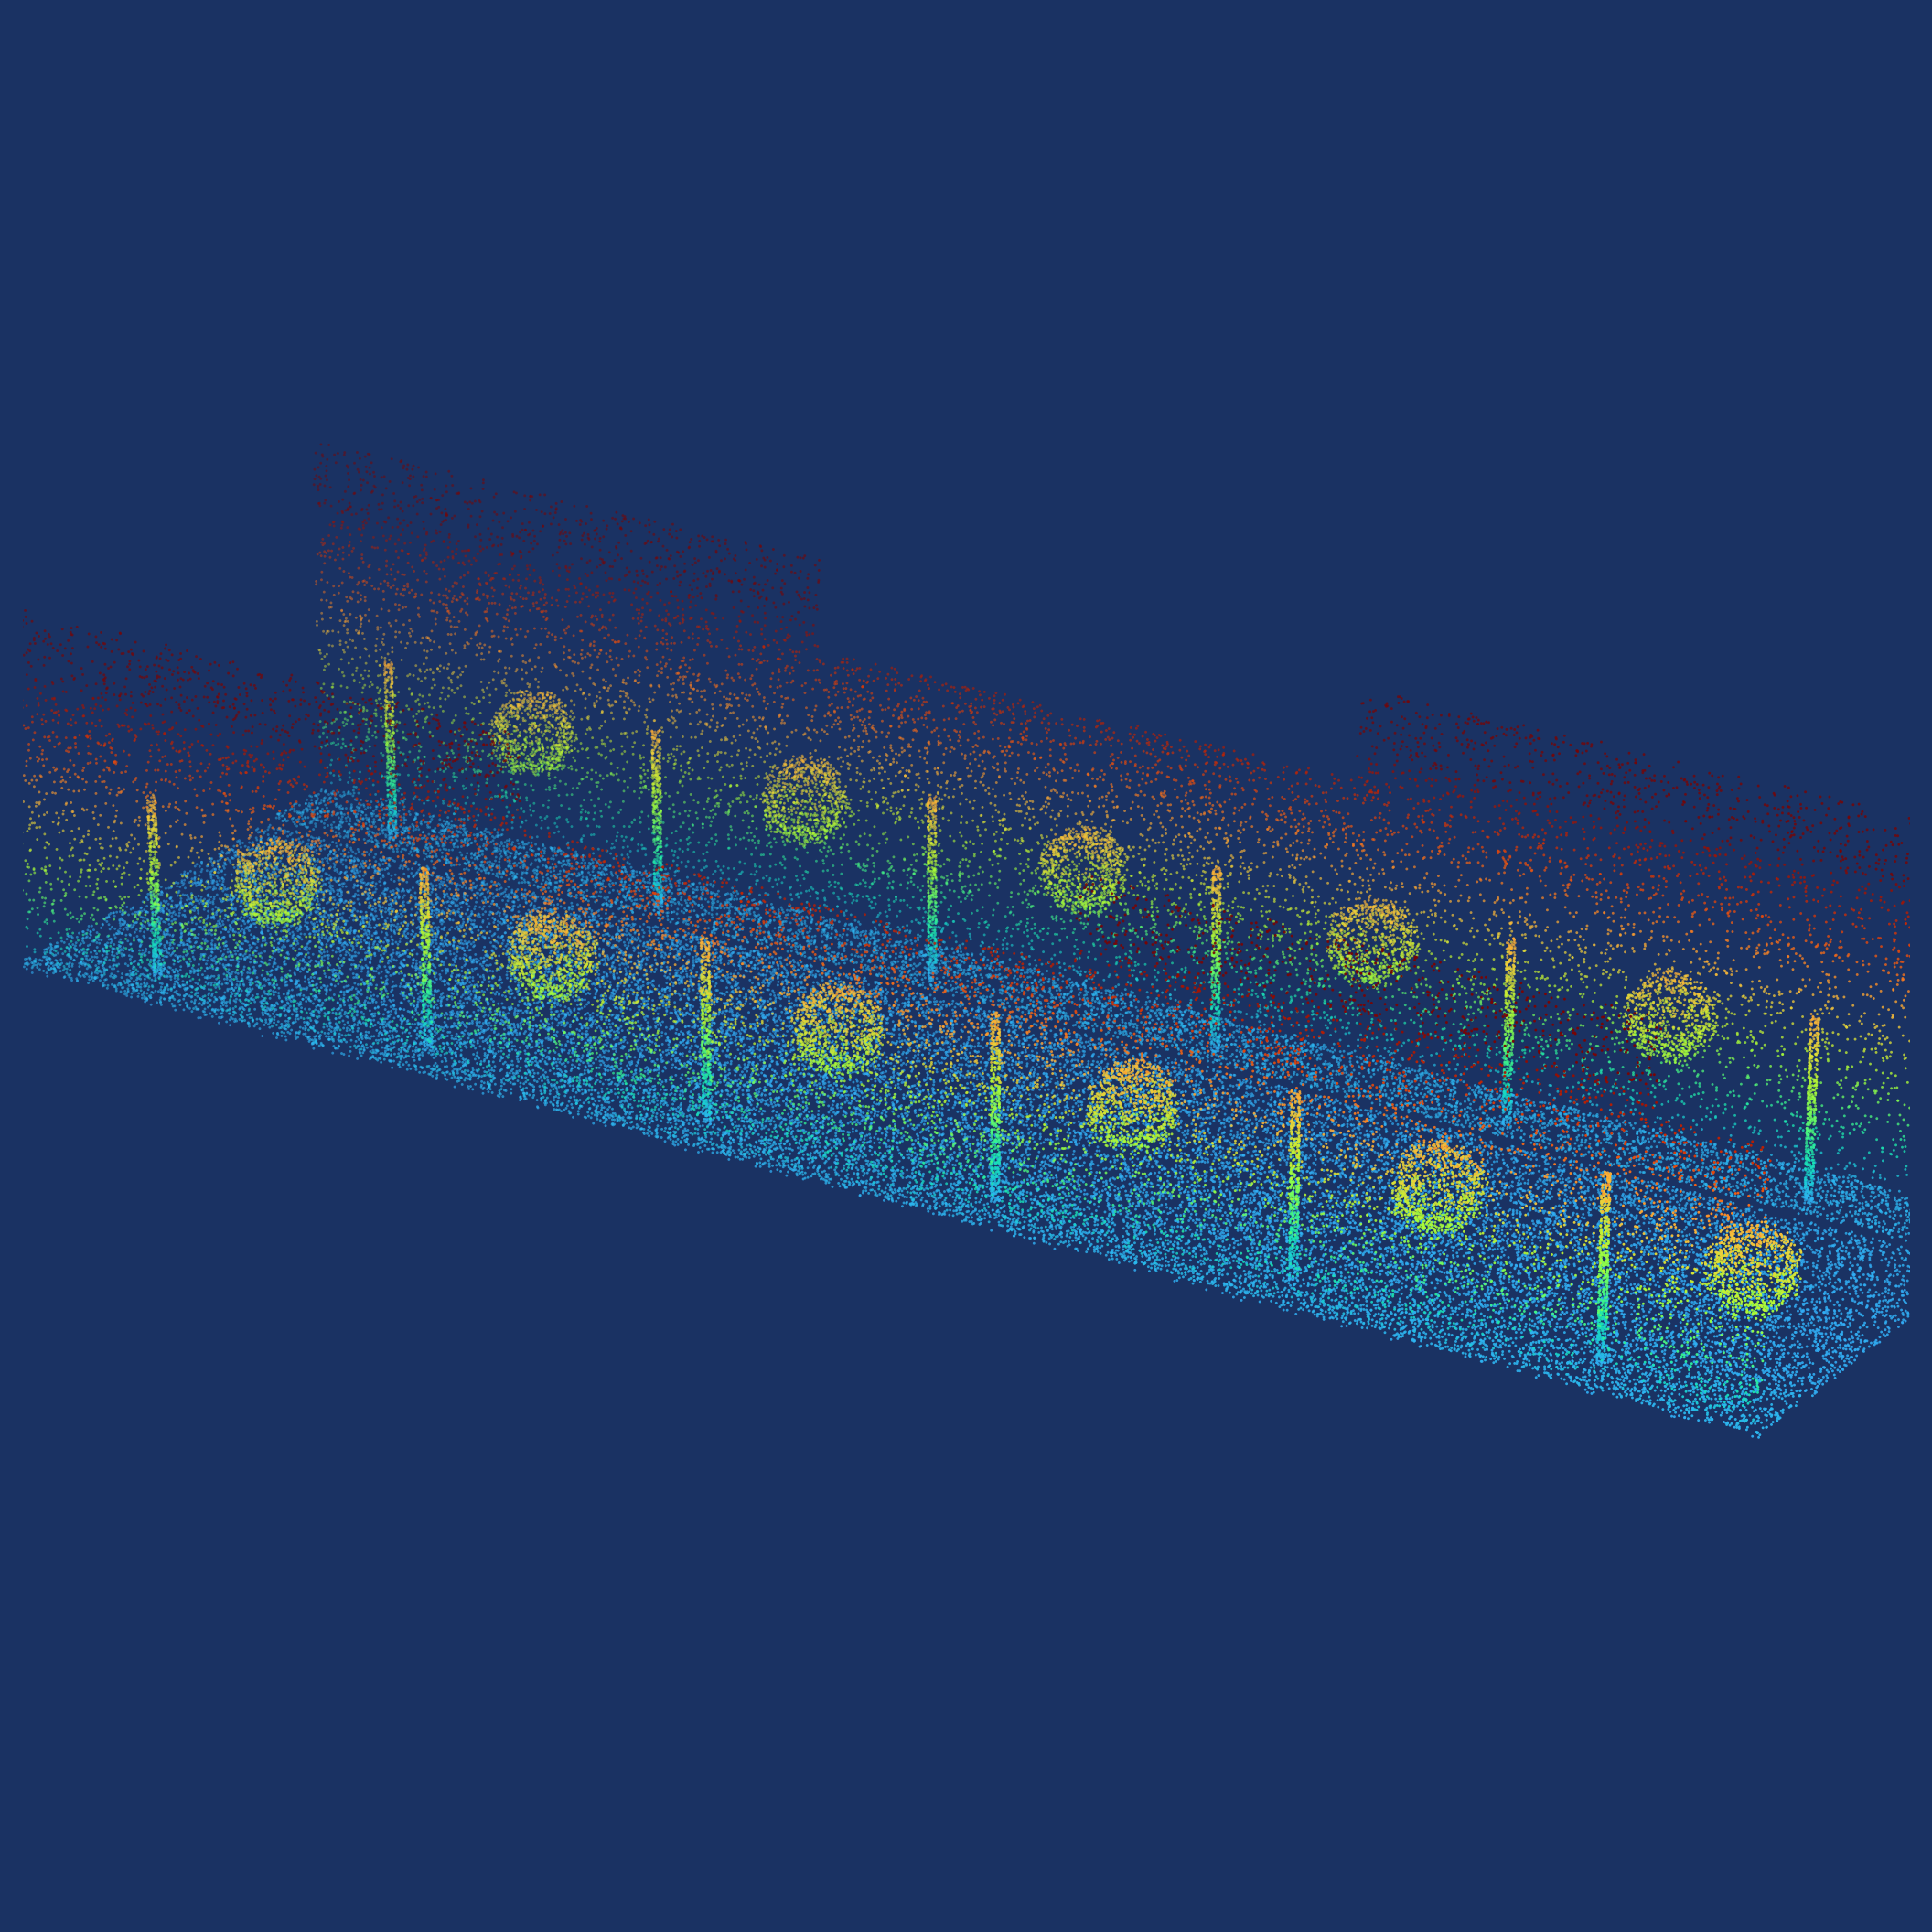
\includegraphics[width=\paperwidth]{cover}};
\fill[orange] ([yshift=-3.05in]current page.north west) rectangle ([yshift=-3.12in]current page.north east);
\node[anchor=north west,text width=7in,align=left] at ([xshift=0.75in,yshift=-0.8in]current page.north west)
 {\color{white}\sffamily\bfseries\fontsize{40}{46}\selectfont\spaceskip=0.28em LiDAR from the Ground Up};
\node[anchor=north west,text width=7in,align=left] at ([xshift=0.75in,yshift=-1.65in]current page.north west)
 {\color{orange!60}\sffamily\Large Mobile Laser Scanning, IMUs, SLAM and Survey-Grade Deliverables};
\node[anchor=north west,text width=7in,align=left] at ([xshift=0.75in,yshift=-2.05in]current page.north west)
 {\color{white}\sffamily\bfseries\LARGE D.S. Banks, PSM};
\node[anchor=north west,text width=7in,align=left] at ([xshift=0.75in,yshift=-2.55in]current page.north west)
 {\color{white!85}\sffamily\large A two-track course: a simple approach anyone can follow,\\ and a rigorous engineering treatment --- on every topic.};
\node[anchor=south west,text width=7in,align=left] at ([xshift=0.75in,yshift=0.8in]current page.south west)
 {\color{white}\sffamily\large 21 modules \textbullet\ 85+ illustrations \textbullet\ 80+ fully worked examples \textbullet\ every equation explained\\[6pt]
 \color{white!70}\sffamily\normalsize Course Text \textbullet\ October 2026};
\end{tikzpicture}
\end{titlepage}

\chapter*{How to Use This Course}
\markboth{How to Use This Course}{}
This course teaches mobile LiDAR --- the technology that lets a car, a backpack or a drone measure millions of 3-D points while it moves --- from the very first idea (``light bounces back'') all the way to the factor-graph mathematics inside modern SLAM software such as LIO-SAM, and the accuracy statistics a surveyor signs off on.

It was built by pulling together three source documents --- a four-module course outline, a 59-page \emph{Mobile LiDAR Basics} seminar, and the LIO-SAM research paper (Shan \emph{et al.}, 2020) --- then reorganizing, correcting and greatly expanding them. Wherever we fixed or sharpened something from those sources you will see a red \emph{Improved from the source material} box, so you can see exactly what changed and why.

\section*{Two readers, one book}
Every module is written on two levels at the same time. You can read only one track, or both.

\begin{kid}
Green boxes like this one take the simple approach: they explain the idea with everyday objects and familiar experiences. No algebra is needed. If you want the picture in your head before the math, read these first.
\end{kid}

\begin{eng}
Blue boxes give the precise statement: the governing equations, the assumptions behind them, the conventions, and how the idea connects to surveying practice, standards and software.
\end{eng}

\section*{The other boxes}
\begin{keyeq}{Name of the equation}
Every important equation is framed like this, and is \emph{always} followed by a table called \textbf{What every symbol means} --- each letter, what it stands for, and its units. No symbol is ever left unexplained.
\end{keyeq}

\begin{worked}{a fully solved problem}
Orange boxes solve a realistic problem step by step: \emph{Given}, then numbered steps with every bit of arithmetic shown, then the \emph{Result}. All numbers in this book were checked by computer.
\end{worked}

\begin{tryit}
Purple boxes give you a problem to solve on your own. Answers are at the back of the book (Appendix A).
\end{tryit}

\begin{tip}
Teal boxes connect the idea to real field and office practice for surveyors and civil engineers.
\end{tip}

\begin{seminar}
If you are taking this course as a \textbf{survey seminar} (for example, for continuing-education credit), here is exactly what you are responsible for:
\begin{itemize}
\item \textbf{You are responsible for the graphs and the concepts.} Read the Simple Approach boxes, the Engineer's View text, the figures and their captions, the Surveyor's Field Tips, the Big Ideas, and the Improved From the Source Material boxes. You should be able to explain what each graph shows and why it matters in the field.
\item \textbf{You are not responsible for the equations.} The Key Equation boxes, the arithmetic inside the Worked Examples, the Try It Yourself problems, and Appendices A and C are there for engineers and for reference. Skim them for the story they tell; you will not be asked to reproduce or solve them.
\item \textbf{All exam questions are conceptual and standards related.} The final exam is \textbf{not printed in this book}: the instructor administers it from a separate instructor packet (two versions). It has no calculations and needs no calculator. The \textbf{pass mark is 70\%}. It tests the ideas behind LiDAR, IMUs, SLAM and error propagation, and the professional standards discussed in the course: the ASPRS Positional Accuracy Standards (Edition 2), the Florida Standards of Practice (Chapter 5J-17, F.A.C.), FDOT TML requirements, the NSRS modernization, FAA Part 107, laser eye safety, control versus checkpoints, datums and documentation of the work.
\end{itemize}
\textbf{Suggested path:} follow the six-hour agenda below; give extra attention to Modules 13--14 (accuracy standards and error budgets), 19--20 (Florida standards and professional practice) and 21 (capstone and sample dataset); study the sample SOP and client accuracy agreement in Appendix E.
\end{seminar}


\section*{Six-hour seminar agenda}
\begin{center}\small
\renewcommand{\arraystretch}{1.22}
\begin{tabularx}{\linewidth}{>{\bfseries}p{2.4cm}X>{\raggedright\arraybackslash}p{3.4cm}}\toprule
Time & Topic & Modules\\\midrule
0:00--0:15 & Welcome, objectives, how the course works & front matter\\
0:15--1:00 & What LiDAR measures; light, beam, reflectivity, what it can see through & 1, 3, 4, 5\\
1:00--1:45 & Pose, the right-hand rule, IMUs, timing, calibration & 6, 7, 8, 9\\
1:45--2:00 & Break & \\
2:00--2:45 & SLAM, scan matching, factor graphs; how the trajectory is built & 10, 11, 12\\
2:45--3:30 & Accuracy standards (ASPRS Edition 2) and error budgets & 13, 14\\
3:30--4:00 & Lunch & \\
4:00--4:45 & Case studies: OS0, GX5/GQ7, RIEGL at 500 ft & 15, 16, 17\\
4:45--5:30 & Processing, Florida standards, professional practice & 18, 19, 20\\
5:30--5:45 & Capstone and sample dataset walk-through & 21, App.\ E\\
5:45--6:15 & Final exam (conceptual, 50 questions, 70\% to pass) and evaluation & instructor packet\\\bottomrule
\end{tabularx}\end{center}
{\footnotesize Six hours of instruction plus breaks; adjust to the approving board's contact-hour rules. Module 2 (math toolkit) is optional reading for seminar participants.}

\section*{Learning objectives}
After the seminar, participants will be able to:
\begin{enumerate}[leftmargin=*]
\item explain how a LiDAR measures range and position and what it can and cannot see (Modules 1--5);
\item describe pose, the right-hand rule and how IMU, LiDAR scans and GNSS build a trajectory (Modules 6--12);
\item interpret accuracy statements and checkpoint tests under ASPRS Edition 2 (Module 13);
\item read an error budget and identify the dominant error source for a given system and range (Modules 14--17);
\item apply Florida 5J-17, FDOT TML and NSRS-modernization requirements to a LiDAR deliverable (Module 19);
\item identify professional-practice obligations: responsible charge, sealing digital data, scope, Part 107, safety and records (Module 20);
\item evaluate a sample project's trajectory, checkpoint table and accuracy report (Module 21).
\end{enumerate}

\section*{What you need}
For seminar participants and the simple track: curiosity --- no calculator is needed. For the engineer's track: algebra, a little trigonometry (Module 2 teaches all of it from scratch), and a scientific calculator. Matrices appear from Module 6 onward and are explained as they arrive.

\section*{Course map}
\begin{center}\small\sffamily
\renewcommand{\arraystretch}{1.25}
\begin{tabularx}{\linewidth}{>{\bfseries}lX>{\raggedright\arraybackslash}p{4.4cm}}
\toprule
Part & Modules & Source outline module \\ \midrule
A & 1 What is LiDAR? \textbullet\ 2 Math toolkit & --- (foundation) \\
B & 3 Time of flight \textbullet\ 4 The beam \textbullet\ 5 Angles to X,Y,Z & Module 1: Sensor architecture \\
C & 6 Rotation \& pose \textbullet\ 7 IMU \textbullet\ 8 Timing \& motion compensation & Module 1: IMUs, time sync \\
D & 9 Lever arm \& boresight calibration & Module 3: System calibration \\
E & 10 SLAM \textbullet\ 11 Scan matching \textbullet\ 12 Factor graphs \& LIO-SAM & Module 2: SLAM \& trajectory \\
F & 13 Control \& accuracy standards \textbullet\ 14 Error propagation \& all error budgets & Module 3: Control \& error propagation \\
G & Short case studies: 15 Ouster OS0 \textbullet\ 16 GX5-25 / GX5-45 / GQ7 \textbullet\ 17 RIEGL VUX-240\textsuperscript{24} & Module 1: Sensors \& IMUs (applied) \\
H & 18 Processing \& deliverables \textbullet\ 19 Florida standards, FDOT \& NSRS \textbullet\ 20 Professional practice \textbullet\ 21 Capstone \& sample dataset & Module 4: Workflows \& QA/QC; Florida practice \\
\bottomrule
\end{tabularx}
\end{center}

\tableofcontents
\mainmatter
